\documentclass[a4j,10pt]{jarticle}
\title{電気回路}
\author{高浜 陸生}
\date{2013年4月20日}
\usepackage{slashbox}
\usepackage[dvipdfm]{graphicx}
\newcommand{\Tabref}[1]{表~(\ref{#1})}
\newcommand{\Equref}[1]{式~(\ref{#1})}
\newcommand{\Figref}[1]{図~(\ref{#1})}
\begin{document}
\section{目的}
今回の実験では、コンデンサとコイル、抵抗を接続した直列回路に電流を流し、
その際に現れる減衰波形を観測することが目的である。
また、観測した波形から電気回路の中で起こった力学的現象について観察し、
減衰振動の周波数やピーク電圧などと時間の関係について考察する。
\section{原理}
直列に抵抗のみをつないだ回路における電流$I(t)$や電圧$V_{R}(t)$は、
Ohmの法則により\Equref{Ronly}で表される。
\begin{eqnarray}
\label{Ronly}
V_{R}(t)=RI(t)
\end{eqnarray}
コンデンサが直流電源で充電されている場合を考える。コンデンサの静電容量をCとすると、
コンデンサに蓄えられている電荷$q(t)$と両端電圧$V_{C}(t)$との関係は\Equref{Conly}で表される
\begin{eqnarray}
\label{Conly}
q(t)=CV_{C}(t)
\end{eqnarray}
また、電流は単位時間辺りにある面を通過する電荷の量で表されるので、
\begin{eqnarray}
I(t)=\frac{dq(t)}{dt}
\end{eqnarray}
となる。
コイルは時間変化する電流に対して誘導起電力を生じる。コイルの自己インダクタンスL、ある時間tにおけるコイルへの流入電流を$I(t)$とすると、
誘導起電力$V_{L}(t)$は\Equref{Lind}で表される。
\begin{eqnarray}
\label{Lind}
V_{L}(t)=-L\frac{dI(t)}{dt}
\end{eqnarray}
次に、抵抗、コイル、コンデンサを直列につないだ回路に直流電源を接続した場合に回路に流れる電流について考える。
電源の起電力をVとし、ある時刻tにおいて、コンデンサに蓄えられている電荷$q(t)$、抵抗値、インダクタンスと静電容量をそれぞれR、L、C、とすると、
回路に流れる電流$I(t)$は\Equref{RLC:1}を満たす。
\begin{eqnarray}
\label{RLC:1}
V-L\frac{dI(t)}{dt}=RI(t)+\frac{q(t)}{C}
\end{eqnarray}
\Equref{RLC:1}の両辺を時間で微分し、\Equref{Conly}を用い$2\gamma=R/L$,$\omega_{0}^{2}=1/(LC)$とおくと、
\begin{eqnarray}
\label{RLC:2}
\frac{d^2I(t)}{dt^{2}}+2\gamma\frac{dI(t)}{dt}+\omega_{0}^{2}I(t)=0
\end{eqnarray}
と表すことができる。//
また、\Equref{RLC:2}の$I(t)$を$x(t)$に置き換えると、速度に比例する抵抗力が働く単振動の運動方程式と同形であり、
解は$\gamma$と$\omega_{0}^{2}$の大小関係により次の3つに分かれることが知られている。
\begin{description}
\item[(i)]$\gamma<\omega_{0}$(減衰振動)
\begin{eqnarray}
\label{freq}
				I(t)=e^{-{\gamma}t}(a\sin\omega_{1}t+b\cos\omega_{1}t)
\end{eqnarray}
\item[(ii)]$\gamma>\omega_{0}$(過減衰)
\begin{eqnarray}
\label{over}
				I(t)=e^{-{\gamma}t}(ae^{\omega_{1}t}+be^{\omega_{1}t}
\end{eqnarray}
\item[(iii)]$\gamma=\omega_{0}$(臨界減衰)
\begin{eqnarray}
\label{critical}
				I(t)=e^{-{\gamma}t}(at+b)
\end{eqnarray}
\end{description}

ここで、a,bはいずれも初期条件で定まる定数、また角周波数$\omega_{1}$は、過減衰の場合
$\omega_{1}=\sqrt{\gamma^{2}-\omega_{0}^{2}}$、減衰振動の場合$\omega_{1}=\sqrt{\omega_{0}^{2}-\gamma^{2}}$となる。
回路を組み、時間と電流の関係を観測することで角周波数$\omega_{0}$や抵抗係数$\gamma$を求めることができる。
\section{実験方法}
実験方法は以下のとおりである。
\begin{enumerate}

\item 必要な素子の選出\\
ブレッドボードにあらかじめ設置されているコイルのインダクタンスLをLCRメータで測り、記録しておく。
次に$10[\mathrm k \Omega]$の抵抗をつないだと仮定し、コンデンサを含めRLC回路を組んだ際に臨界減衰が起こるような
静電容量Cを計算する。
計算によって求められた静電容量Cに近い値のコンデンサをボックスから選び、次の実験を行う。
\item 減衰振動の測定\\
部品箱から$100~200[\Omega]$の抵抗を選びテスタで測定し、オシロスコープと発振器を次の手順にしたがい設定する。


\begin{itemize}
\item 発振器の発信波形を矩形波に、発信周波数は100[Hz]に設定する。
\item 発振器のAMPL(振幅調整)つまみを全体の1/2程度回す。
\item オシロスコープのトリガをAUTOに設定し、自動でトリガを検出するようにする。
\item VOLT/DIV,TIME/DIVを適当な大きさに設定し、波形が見やすい大きさとなるようにする。
\item 適切な波形が観測できるようになったらSTOPボタンを押し、波形を止める。
\end{itemize}


なお、減衰振動やこの後に行う過減衰の測定においても、波形は一回分の波形を表示するように調整を行うこと。
観測しやすい波形を得られたならば次の作業を行う。
\begin{itemize}
\item USBメモリにBMPとして保存か、グラフ用紙にスケッチするかどちらかの方法で波形を記録する。
手書きする場合は、1[mm]方眼紙にスケッチし、縦軸横軸の感度値も忘れずに記録しておく。
また、スケッチする場合は波形のピーク値と時間の関係が読み取れるよう心がけること。
\item オシロスコープのカーソル機能を使用し波形のピーク時の時間と電圧の関係を読み取る。
\item 上記の測定値を周期とし、波形の周波数を算出、\Equref{freq}の$\omega_{1}$の値と比較し概ね正しい値となっていることを確認する。
		大きく違う場合は測定を間違えている可能性が高い。
\end{itemize}
\item 過減衰の測定
抵抗値$20[\mathrm k \Omega]$の抵抗を選びテスタで測定、抵抗値を記録しておく。減衰振動と同様に波形を保存またはスケッチした後、
時間軸1[DIV]ごとの電圧値をカーソル機能を使い測定する。
\end{enumerate}
時間が余った場合は抵抗値を変え測定を繰り返し行う。
\section{実験器具}
今回使用した実験器具のリストは表(1)となっている。
\begin{table}[hc]
\caption{使用機器}
\begin{tabular}{|l|c|r|r|}
\hline
名称 & メーカー & 型番 & 製造番号 \\ \hline \hline
オシロスコープ & INSTEK & DS-5404B & AF104100433 \\ \hline
Function Generator & IWATSU & SFG-2004 & EK892481 \\ \hline
プローブ&KENWOOD&PC-54&  \\ \hline
テスタ&IWATSU&VOAC-21& \\ \cline{2-4}
&AND&AD5827&0860640183 \\ \hline
\end{tabular}
\end{table}
\section{結果}
コイルのインダクタンスは$L=202.3\times10^{-3}[\mathrm H]$,
これより計算したコンデンサの静電容量の値は$C=8.092\times10^{-9}[\mathrm C]$,これにもっとも近い値として
$10\times10^{-9}[\mathrm C]$のものを使用した。

減衰振動の実験のデータは表(2)、波形は図(1)となった。
\begin{figure}[h]
\begin{center}
\label{Gensui}
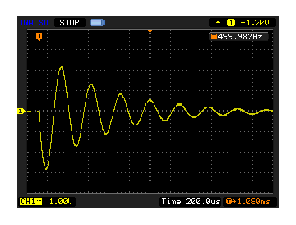
\includegraphics[width=5cm]{freq.eps}
\caption{減衰振動の波形}
\end{center}
\end{figure}
\begin{table}[h]
\begin{center}
\caption{減衰振動における測定データ}
\begin{tabular}{|l|r|r|r|}
\hline
回数 & 時間$t_{1}[\mu \mathrm s]$ & 電圧$V_{i}[\mathrm V]$ & 電圧比の対数 \\ \hline \hline
1 & 76 & 2.76 & None \\ \hline
2 & 220 & 2.16 & -0.106 \\ \hline
3 & 368 & 1.68 & -0.109 \\ \hline
4 & 514 & 1.36 & -0.092 \\ \hline
5 & 656 & 1.04 & -0.116 \\ \hline
6 & 800 & 0.840 & -0.093 \\ \hline
7 & 944 & 0.640 & -0.118 \\ \hline
8 & 1090 & 0.400 & -0.204 \\ \hline
\end{tabular}
\end{center}
\end{table}

また、表(2)のグラフは巻末図(2)にある。

過減衰の実験において、抵抗は$22.886[\mathrm k \Omega]$のものを使用した。
過減衰のグラフは図(3)、データは表(3)となっている。
\begin{figure}[h]
\begin{center}
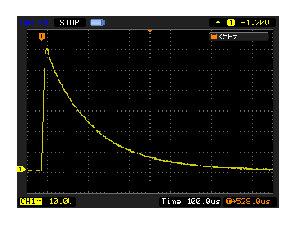
\includegraphics[width=5cm]{over.eps}
\caption{過減衰の波形}
\end{center}
\end{figure}
\begin{table}[h]
\begin{center}
\caption{グラフ一目盛あたりの電圧}
\begin{tabular}{|l|r|}
\hline
n[DIV]&$V_{i}[\mathrm V]$ \\ \hline \hline
1&58.8 \\ \hline
2&38.8 \\ \hline
3&14.0 \\ \hline
4&8.8  \\ \hline
5&5.6  \\ \hline
6&3.6  \\ \hline
7&3.2  \\ \hline
8&1.2  \\ \hline
\end{tabular}
\end{center}
\end{table}
表(3)のグラフは巻末図(3)となっている。
\section{考察}

\end{document}
